%%%%(c) COPYRIGHT NOTICE%FOLDUP
%%%%(c)
%%%%(c)  This file is a portion of the source for the textbook
%%%%(c)
%%%%(c)    Numerical Methods Course Notes,
%%%%(c)    Copyright 2004-2010 by Steven E. Pav
%%%%(c)
%%%%(c)  See the file COPYING.txt for copying conditions
%%%%(c)
%%%%(c)%UNFOLD

%%throat clearing%FOLDUP
\typeout{-- splines.tex}
\typeout{-- N� 2004-2010 Steven E. Pav}
%UNFOLD

%%local commands%FOLDUP
%UNFOLD

\chapter{Spline Interpolation}

\index{splines}%
Splines are used to approximate complex functions and shapes.  A spline
is a function consisting of simple functions glued together.  In this way a
spline is different from a polynomial interpolation, which consists of a single
well defined function that approximates a given shape;  splines are normally
piecewise polynomial.  

%%%%%%%%%%%%%%%%%%%%%%%%%%%%%%%%%%%%%%%%%%%%%%%
\section{First and Second Degree Splines}%FOLDUP

Splines make use of partitions, which are a way of cutting an interval into a
number of subintervals.

\begin{bkdefinition}[Partition]
A \emph{partition} of the interval \ccinv{a}{b} is an ordered sequence
\setBIdx{t_i}{i=0}{n} such that
\[a = t_0 < t_1 < \cdots < t_{n-1} < t_n = b\]
The numbers $t_i$ are known as \emph{knots}.
\index{partition}\index{knot}%
\end{bkdefinition}

A spline of degree 1, also known as a \emph{linear spline}, is a function which is linear on each subinterval defined
by a partition:\index{splines!linear}

\begin{bkdefinition}[Linear Splines]
A function $S$ is a spline of degree $1$ on \ccinv{a}{b} if
\begin{compactenum}
\item The domain of $S$ is \ccinv{a}{b}.
\item $S$ is continuous on \ccinv{a}{b}.
\item There is a partition \setBIdx{t_i}{i=0}{n} of \ccinv{a}{b} such that on
each \ccinv{t_i}{t_{i+1}}, $S$ is a linear polynomial.
\end{compactenum}
\end{bkdefinition}

A linear spline is defined entirely by its value at the knots.  That is,
given
\[\begin{array}{c|*{4}{|c}}
t & t_0 & t_1 & \ldots & t_n\\
\hline
y & y_0 & y_1 & \ldots & y_n
\end{array}\]
there is only one linear spline with these values at the knots and linear on
each given subinterval.

For a spline with this data, the linear polynomial on each subinterval is
defined as
\[S_i(x) = y_i + \frac{y_{i+1} - y_{i}}{t_{i+1} - t_{i}} \Parens{x - t_i}.\]
Note that if $x \in \ccinv{t_i}{t_{i+1}},$ then $x - t_i > 0,$ but $x - t_{i-1}
\le 0.$  Thus if we wish to evaluate $S(x),$ we search for the largest $i$ such that 
$x - t_i > 0,$ then evaluate $S_i(x).$

\begin{bkexample}%FOLDUP
The linear spline for the following data
\[\begin{array}{c|*{6}{|c}}
t & 0.0  & 0.1  & 0.4  & 0.5  & 0.75 & 1.0\\
\hline
y & 1.3 & 4.5 & 2.0 & 2.1 & 5.0 & 3 
\end{array}\]
is shown in \figref{splineone}.
%\figref{splineone}%FOLDUP
\begin{figure}[htb!]
\centering
	\includegraphics[height=0.65\columnwidth,angle=270,clip=]{spline1.eps}
\caption{A linear spline.  The spline is piecewise linear, and is linear 
between each knot.}\label{fig:splineone}
\end{figure}%UNFOLD
\end{bkexample}
%UNFOLD

%%%%%%%%%%%%%%%%%%%%%%%%%%%%%%%%%%%%%%%%%%%%%%%
\subsection{First Degree Spline Accuracy}%FOLDUP

As with polynomial functions, splines are used to interpolate tabulated data as
well as functions.  In the latter case, if the spline is being used to interpolate
the function $f,$ say, then this is equivalent to interpolating the data
\[\begin{array}{c|*{4}{|c}}
t & t_0 & t_1 & \ldots & t_n\\
\hline
y & f(t_0) & f(t_1) & \ldots & f(t_n)
\end{array}\]

A function and its linear spline interpolant are shown in
\figref{splinterp}.  The spline interpolant in that figure is fairly close to
the function over some of the interval in question, but it also deviates
greatly from the function at other points of the interval.
We are interested in finding bounds on the possible error between a function and its
spline interpolant.

%\figref{splinterp}%FOLDUP
\begin{figure}[htb!]
\centering
	\psfrag{fn}[Br][r][0.65]{function}
	\psfrag{interp}[Br][r][0.65]{spline interpolant}
	\includegraphics[height=0.65\columnwidth,angle=270,clip=]{splinterp.eps}
\caption{The function $f(t) = 4.1 + \sin \oneBy{(0.08 t + 0.5)}$ is shown, along
with the linear spline interpolant, for the knots $0, 0.1, 0.4, 0.6,
0.75, 0.9, 1.0$  For some values of $t,$ the function and its interpolant are
very close, while they vary greatly in the middle of the interval.}\label{fig:splinterp}
\end{figure}%UNFOLD


To find the error bound, we will consider the error on a single interval of the
partition, and use a little calculus.\footnote{Although we could directly claim
\thmref{interror}, it is a bit of overkill.}
Suppose $p(t)$ is the linear polynomial interpolating $f(t)$ at the
endpoints of the subinterval \ccinv{t_i}{t_{i+1}}, then for $t \in
\ccinv{t_i}{t_{i+1}},$ 
\[\abs{f(t) - p(t)} \le \max\sngtn{\abs{f(t) - f(t_i)},\abs{f(t) - f(t_{i+1})}}.\]
%
That is, $\abs{f(t) - p(t)}$ is no larger than the ``maximum variation'' of $f(t)$
on this interval.  

In particular, if $f'(t)$ exists and is bounded by $M_1$ on \ccinv{t_i}{t_{i+1}}, then
\[\abs{f(t) - p(t)} \le \frac{M_1}{2} \Parens{t_{i+1}-t_i}.\]
Similarly, if $f''(t)$ exists and is bounded by $M_2$ on \ccinv{t_i}{t_{i+1}}, then
\[\abs{f(t) - p(t)} \le \frac{M_2}{8} \Parens{t_{i+1}-t_i}^2.\]
%
%\begin{proof}
%Let $g(t)$ be a function such that $g(t_i) = g(t_{i+1}) = 0,$ and such that
%$\abs{g'(t)} \le \hat{M}_1$ for $t \in \ccinv{t_i}{t_{i+1}}.$  
%Consider the case where $t-t_i \le t_{i+1} - t.$  Then
%\[\abs{g(t) - g(t_i)} = \abs{g(t)} = \abs{\int_{t_i}^{t} g'(t) \dx[t]} \le
%\int_{t_i}^{t} \abs{g'(t)}\dx[t] \le 
%\int_{t_i}^{t} \hat{M}_1 \dx[t] 
%= \hat{M}_1 \abs{t - t_i}
%\le \frac{\hat{M}_1}{2} \abs{t - t_i}
%\]
%Consider the case where $t-t_i \le t_{i+1} - t.$  Then
%\[\abs{f(t) - p(t)} = \abs{\int_{t_i}^{t} f'(t) - p'(t)\dx[t]} \le 
% \int_{t_i}^{t} \abs{f'(t) - p'(t)} \dx[t] \le 
%\]
%\end{proof}

Over a given partition, these become, respectively

\begin{empheq}[innerbox=\widefbox]{equation}
\begin{split}
\abs{f(t)-p(t)} &\le \frac{M_1}{2} \max\limits_{0\le i < n}
\Parens{t_{i+1}-t_i},\\
\abs{f(t)-p(t)} &\le \frac{M_2}{8} \max\limits_{0\le i < n}
\Parens{t_{i+1}-t_i}^2.
\end{split}
\end{empheq}

If equally spaced nodes are used, these bounds guarantee that spline
interpolants become better as the number of nodes is increased.
This contrasts with polynomial interpolants, which may get worse as the
number of nodes is increased, \cf \bkexref{rungef}.

%UNFOLD

%%%%%%%%%%%%%%%%%%%%%%%%%%%%%%%%%%%%%%%%%%%%%%%
\subsection{Second Degree Splines}%FOLDUP

Piecewise quadratic splines, or splines of degree 2, are defined
similarly:\index{splines!quadratic}

\begin{bkdefinition}[Quadratic Splines]
A function $Q$ is a quadratic spline on \ccinv{a}{b} if
\begin{compactenum}
\item The domain of $Q$ is \ccinv{a}{b}.
\item $Q$ is continuous on \ccinv{a}{b}.
\item $Q'$ is continuous on \ooinv{a}{b}.
\item There is a partition \setBIdx{t_i}{i=0}{n} of \ccinv{a}{b} such that on
\ccinv{t_i}{t_{i+1}}, $Q$ is a polynomial of degree at most 2.
\end{compactenum}
\end{bkdefinition}

\begin{bkexample}
The following is a quadratic splne:
\[Q(x) = \left\{ \begin{array}{rl}
	-x & x\le0,\\
	x^2 - x & 0\le x \le 2,\\
	-x^2 + 7 x -8 & 2\le x.\end{array}\right.\]
\end{bkexample}

Unlike linear splines, quadratic splines are \emph{not} defined entirely by
their values at the knots.  We consider why that is.  The spline $Q(x)$ is
defined by its piecewise polynomials, 
\[Q_i(x) = a_i x^2 + b_i x + c_i.\]
Thus there are $3n$ parameters to define $Q(x).$

For each of the $n$ subintervals, the data
\[\begin{array}{c||c|c|c|c}
t & t_0 & t_1 & \ldots & t_n\\
\hline
y & y_0 & y_1 & \ldots & y_n
\end{array}\]
give two equations regarding $Q_i(x),$ namely that $Q_i(t_i)$ must equal $y_i$
and $Q_i(t_{i+1})$ must equal $y_{i+1}.$  This is $2n$ equations.
The condition on continuity of $Q'$ gives a single equation for each of the
$n-1$ internal nodes.  This totals $3n-1$ equations, but $3n$ unknowns.  This
system is underdetermined.

Thus some additional user-chosen condition is required to determine the
quadratic spline.  One might choose, for example, $Q'(a) = 0,$ or $Q''(a) = 0,$
or some other condition.


%UNFOLD

%%%%%%%%%%%%%%%%%%%%%%%%%%%%%%%%%%%%%%%%%%%%%%%
\subsection{Computing Second Degree Splines}\label{subsec:compsplinetwo}%FOLDUP

Suppose the data
\[\begin{array}{c||c|c|c|c}
t & t_0 & t_1 & \ldots & t_n\\
\hline
y & y_0 & y_1 & \ldots & y_n
\end{array}\]
are given.  Let $z_i = Q'_i(t_i),$ and suppose that the additional condition to
define the quadratic spline is given by specifying $z_0.$  We want to be able
to compute the form of $Q_i(x).$

Because $Q_i(t_i) = y_i, Q'_i(t_i) = z_i,Q'_i(t_{i+1}) = z_{i+1},$ we see that
we can define
\[
Q_i(x) = \frac{z_{i+1} - z_i}{2\Parens{t_{i+1} - t_i}} \Parens{x - t_i}^2 + z_i\Parens{x - t_i} + y_i.
\]
Use this at $t_{i+1}:$
\begin{align*}
y_{i+1} = Q_i(t_{i+1}) &= \frac{z_{i+1} - z_i}{2\Parens{t_{i+1} - t_i}} \Parens{t_{i+1} - t_i}^2 + z_i\Parens{t_{i+1} - t_i} + y_i,\\
 y_{i+1} - y_i &= \frac{z_{i+1} - z_i}{2} \Parens{t_{i+1} - t_i} + z_i\Parens{t_{i+1} - t_i},\\
 y_{i+1} - y_i &= \frac{z_{i+1} + z_i}{2} \Parens{t_{i+1} - t_i}.
\end{align*}
Thus we can determine, from the data alone, $z_{i+1}$ from $z_i$:
\begin{equation*}
z_{i+1} =  2\frac{y_{i+1} - y_i}{t_{i+1} - t_i} - z_i.
\end{equation*}


%UNFOLD
%UNFOLD
%%%%%%%%%%%%%%%%%%%%%%%%%%%%%%%%%%%%%%%%%%%%%%%
\section{(Natural) Cubic Splines}%FOLDUP

If you recall the definition of the linear and quadratic splines, probably you
can guess the definition of the spline of degree $k$:

\begin{bkdefinition}[Splines of Degree k]
A function $S$ is a spline of degree $k$ on \ccinv{a}{b} if
\begin{compactenum}
\item The domain of $S$ is \ccinv{a}{b}.
\item $S,S',S'',\ldots,S^{(k-1)}$ are continuous on \ooinv{a}{b}.
\item There is a partition \setBIdx{t_i}{i=0}{n} of \ccinv{a}{b} such that on
\ccinv{t_i}{t_{i+1}}, $S$ is a polynomial of degree $\le k.$
\end{compactenum}
\end{bkdefinition}

You would also expect that a spline of degree $k$ has $k-1$ ``degrees of
freedom,'' as we show here.  If the partition has $n+1$ knots, the spline of 
degree $k$ is defined by $n(k+1)$ parameters.  The given data
\[\begin{array}{c|*{4}{|c}}
t & t_0 & t_1 & \ldots & t_n\\
\hline
y & y_0 & y_1 & \ldots & y_n
\end{array}\]
provide $2n$ equations.  The continuity of $S',S'',\ldots,S^{(k-1)}$ at the
$n-1$ internal knots gives $(k-1)(n-1)$ equations. This is a total of $n(k+1) -
(k-1)$ equations.  Thus we have $k-1$ more unknowns than equations.  Thus,
barring some singularity, we can (and must) add $k-1$ constraints to uniquely
define the spline.  These are the degrees of freedom.

Often $k$ is chosen as $3.$  This yields cubic splines.  We must add $2$ extra
constraints to define the spline.  The usual choice is to make
\[S''(t_0) = S''(t_n) = 0.\]
This yields the \emph{natural cubic spline}.
\index{natural cubic spline}%

%%%%%%%%%%%%%%%%%%%%%%%%%%%%%%%%%%%%%%%%%%%%%%%
\subsection{Why Natural Cubic Splines?}%FOLDUP

It turns out that natural cubic splines are a good choice in the sense that
they are the ``interpolant of minimal $H^2$ seminorm.''
The corollary following this theorem states this in more easily understandable terms:
\begin{bktheorem}
Suppose $f$ has two continuous derivatives, and $S$ is the natural cubic spline
interpolating $f$ at knots $a=t_0 < t_1 < \ldots < t_n = b.$  Then
\[\int_a^b \Bracks{S''(x)}^2 \dx \le \int_a^b \Bracks{f''(x)}^2 \dx\]

\end{bktheorem}
\begin{proof}
We let $g(x) = f(x) - S(x).$  Then $g(x)$ is zero on the $(n+1)$ knots $t_i.$
Derivatives are linear, meaning that 
\[f''(x) = S''(x) + g''(x).\]  Then
\[ \int_a^b \Bracks{f''(x)}^2 \dx =
\int_a^b \Bracks{S''(x)}^2 \dx +
\int_a^b \Bracks{g''(x)}^2 \dx +
\int_a^b 2S''(x)g''(x) \dx .
\]

We show that the last integral is zero.   Integrating by parts we get
\[ \int_a^b S''(x)g''(x) \dx = \dubeval{S''g'}{a}{b} - \int_a^b S'''g'\dx = 
 - \int_a^b S'''g'\dx,\]
because $S''(a) = S''(b) = 0.$  Then notice that $S$ is a polynomial of degree
$\le 3$ on each interval, thus $S'''(x)$ is a piecewise constant function,
taking value $c_i$ on each interval \ccinv{t_i}{t_{i+1}}.  Thus
\[ \int_a^b S'''g'\dx = \sum_{i=0}^{n-1} \int_a^b c_i g' \dx = 
\sum_{i=0}^{n-1} \dubeval{c_i g}{t_i}{t_{i+1}} = 0,\]
with the last equality holding because $g(x)$ is zero at the knots.  
\end{proof}
\begin{bkcorollary}
The natural cubic spline is best twice-continuously differentiable
interpolant for a twice-continuously differentiable function, under the measure
given by the theorem.
\end{bkcorollary}
\begin{proof}
Let $f$ be twice-continuously differentiable, and let $S$ be the natural cubic
spline interpolating $f(x)$ at some given nodes \setBIdx{t_i}{i=0}{n}.  Let
$R(x)$ be some twice-continuously differentiable function which also
interpolates $f(x)$ at these nodes.  Then $S(x)$ interpolates $R(x)$ at these
nodes.  Apply the theorem to get
\[ \int_a^b \Bracks{S''(x)}^2 \dx \le \int_a^b \Bracks{R''(x)}^2 \dx \]
\end{proof}

%UNFOLD

%%%%%%%%%%%%%%%%%%%%%%%%%%%%%%%%%%%%%%%%%%%%%%%
\subsection{Computing Cubic Splines}%FOLDUP
%slightly altered from cheney and kincaid ex 1 in splines 7.2?

First we present an example of computing the natural cubic spline by hand:
\begin{bkexprob}
Construct the natural cubic spline for the following data:
\[\begin{array}{c|*{3}{|c}}
t & -1 & 0 & 2 \\
\hline
y & 3 & -1 & 3
\end{array}\]
\begin{bksolution}
The natural cubic spline is defined by eight parameters:
\[S(x) = \left\{\begin{array}{ll}
	ax^3 + bx^2 + cx + d & x \in \ccinv{-1}{0}\\
	ex^3 + fx^2 + gx + h & x \in \ccinv{0}{2}\end{array}\right.\]
%
We interpolate to find that $d=h=-1$ and
\begin{align*}
-a + b - c - 1 &= 3\\
8e + 4f +2g -1 &= 3
\end{align*}
%
We take the derivative of $S$:
\[S'(x) = \left\{\begin{array}{ll}
	3ax^2 + 2bx + c & x \in \ccinv{-1}{0}\\
	3ex^2 + 2fx + g & x \in \ccinv{0}{2}\end{array}\right.\]
Continuity at the middle node gives $c=g.$
Now take the second derivative of $S$:
\[S''(x) = \left\{\begin{array}{ll}
	6ax + 2b & x \in \ccinv{-1}{0}\\
	6ex + 2f & x \in \ccinv{0}{2}\end{array}\right.\]
Continuity at the middle node gives $b=f.$
The natural cubic spline condition gives $-6a + 2b = 0$ and $12e + 2f = 0$.
Solving this by ``divide and conquer'' gives
%
\[S(x) = \left\{\begin{array}{ll}
	x^3 + 3x^2 -2x - 1 & x \in \ccinv{-1}{0}\\
	-\frac{1}{2}x^3 + 3x^2 -2x - 1 & x \in \ccinv{0}{2}\end{array}\right.\]
\end{bksolution}
\end{bkexprob}

Finding the constants for the previous example was fairly tedious.  And this is
for the case of only three nodes.  We would like a method easier than setting
up the $4n$ equations and unknowns, something akin to the description in
\subsecref{compsplinetwo}.  The method is rather tedious, so we leave it to the
exercises.

%UNFOLD

%UNFOLD
%%%%%%%%%%%%%%%%%%%%%%%%%%%%%%%%%%%%%%%%%%%%%%%
\section{B Splines}%FOLDUP

\index{splines!basis splines}
The B splines form a \emph{basis} for spline functions, whence the name.
We presuppose the existence of an \emph{infinite} number of knots:
\[\ldots < t_2 < t_1 < t_0 < t_1 < t_2 < \ldots,\]
with $\lim_{k\to-\infty} t_k = -\infty$ and $\lim_{k\to\infty} t_k = \infty.$

The B splines of degree 0 are defined as single ``blocks'':
\[B_i^0(x) = \left\{\begin{array}{cl} 1 & t_i \le x < t_{i+1}\\0
&\text{otherwise}\end{array}\right.\]

The zero degree B splines are continuous from the right, are nonzero only on
one subinterval \coinv{t_i}{t_{i+1}}, sum to 1 everywhere.

We justify the description of B splines as basis splines:  If $S$ is a spline
of degree $0$ on the given knots and is continuous from the right then
\[S(x) = \sum_i S(x_i) B_i^0(x).\]
That is, the basis splines work in the same way that Lagrange Polynomials
worked for polynomial interpolation.

The B splines of degree $k$ are defined recursively:
\[
B_i^k(x) = \Parens{\frac{x-t_i}{t_{i+k}-t_i}}B_i^{k-1}(x) + 
 \Parens{\frac{t_{i+k+1} - x}{t_{i+k+1}-t_{i+1}}}B_{i+1}^{k-1}(x).
\]
Some B splines are shown in \figref{somesplines}.

%\figref{somesplines}%%%%%%%%%%%%%%%FOLDUP
\begin{figure}[htbp!]
\begin{center}
\subfigure[Degree 0 B spline]{
	\label{fig:bs0}
	\includegraphics[height=0.45\columnwidth, angle=270,clip=]{bsp0.eps}}
\subfigure[Degree 1 B spline]{
	\label{fig:bs1}
	\includegraphics[height=0.45\columnwidth, angle=270,clip=]{bsp1.eps}}
\subfigure[Degree 2 B spline, with 2 Degree 1 B splines]{
	\label{fig:bs2}
	\psfrag{b10}[Br][r][0.55]{$B_0^1(x)$}
	\psfrag{b11}[Br][r][0.55]{$B_1^1(x)$}
	\psfrag{b20}[Br][r][0.55]{$B_0^2(x)$}
	\includegraphics[height=0.75\columnwidth, angle=270,clip=]{bsp2.eps}}
\end{center}
\caption{Some B splines for the knots $t_0 = 1,t_1 = 2.5,t_2 = 3.5,t_3 = 4$ are shown.  
In (a), one of
the degree 0 B splines; in (b), a degree 1 B spline; in (c), two of the degree
1 B splines and a degree 2 B spline are shown.  The two hat functions ``merge''
together to give the quadratic B spline.}\label{fig:somesplines}
\end{figure}
%UNFOLD

The B splines quickly become unwieldy.  We focus on the case $k=1.$  The B spline
$B_i^1(x)$ is 
\begin{compactitem}
\item Piecewise linear.
\item Continuous.
\item Nonzero only on \ooinv{t_i}{t_{i+2}}.
\item $1$ at $t_{i+1}$.
\end{compactitem}
These B splines are sometimes called \emph{hat functions}.  
Imagine wearing a hat shaped like this!  Whatever.

The nice thing about the hat functions is they allow us to use analogy.  Harken
back to polynomial interpolation and the Lagrange Functions.  The hat functions
play a similar role because
\[B_i^1(t_j) = \delta_{(i+1)j} = \left\{\begin{array}{ll}1 & (i+1)=j\\0 & (i+1)\ne
j\end{array}\right.\]

Then if we want to interpolate the following data with splines of degree 1:
\[\begin{array}{c||c|c|c|c}
t & t_0 & t_1 & \ldots & t_n\\
\hline
y & y_0 & y_1 & \ldots & y_n
\end{array}\]
We can immediately set
\[S(x) = \sum_{i=0}^n y_i B_{i-1}^{1}(x).\]

%UNFOLD
%%%%%%%%%%%%%%%%%%%%%%%%%%%%%%%%%%%%%%%%%%%%%%%
%\section{Exercises}%FOLDUP
\begin{bkexs}
%%%%%%%%%%%%%%%%%%%%%%%%%%%%%%%%
\item Is the following function a linear spline on \ccinv{0}{4}?  Why or why not?
\[S(x) = \begin{cases} 
 3x + 2 &: 0 \le x < 1\\
 -2x + 4 &: 1 \le x \le 4\end{cases}\]
%%%%%%%%%%%%%%%%%%%%%%%%%%%%%%%%
\item Is the following function a linear spline on \ccinv{0}{2}?  Why or why not?
\[S(x) = \begin{cases} 
 x + 3 &: 0 \le x < 1\\
 3 &: 1 \le x \le 2\end{cases}\]
%%%%%%%%%%%%%%%%%%%%%%%%%%%%%%%%
\item Is the following function a linear spline on \ccinv{0}{4}?  Why or why not?
\[S(x) = \begin{cases} 
 x^2 + 3 &: 0 \le x < 3\\
 5x - 6 &: 3 \le x \le 4\end{cases}\]
%%%%%%%%%%%%%%%%%%%%%%%%%%%%%%%%
\item Find constants, $\alpha,\beta$ such that the following is a linear spline
on \ccinv{0}{5}.
\[S(x) = \begin{cases} 
 4x - 2 &: 0 \le x < 1\\
 \alpha x + \beta &: 1 \le x < 3\\
 -2x + 10 &: 3 \le x \le 5\end{cases}\]
%%%%%%%%%%%%%%%%%%%%%%%%%%%%%%%%
\item Is the following function a quadratic spline on \ccinv{0}{4}?  Why or why not?
\[Q(x) = \begin{cases} 
 x^2 + 3 &: 0 \le x < 3\\
 5x - 6 &: 3 \le x \le 4\end{cases}\]
%%%%%%%%%%%%%%%%%%%%%%%%%%%%%%%%
\item Is the following function a quadratic spline on \ccinv{0}{2}?  Why or why not?
\[Q(x) = \begin{cases} 
 x^2 + 3x + 2 &: 0 \le x < 1\\
 2x^2 + x + 3 &: 1 \le x \le 2\end{cases}\]
%%%%%%%%%%%%%%%%%%%%%%%%%%%%%%%%
\item Find constants, $\alpha,\beta,\gamma$ such that the following is a
quadratic spline on \ccinv{0}{5}.
\[Q(x) = \begin{cases} 
 \half x^2 + 2x + \frac{3}{2} &: 0 \le x < 1\\
 \alpha x^2 + \beta x + \gamma &: 1 \le x < 3\\
 3x^2 - 7x + 12 &: 3 \le x \le 5\end{cases}\]
%%%%%%%%%%%%%%%%%%%%%%%%%%%%%%%%
\item Find the quadratic spline that interpolates the following data:
\[\begin{array}{c|*{3}{|c}}
t & 0 & 1 & 4\\
\hline
y & 1 & -2 & 1
\end{array}\]
To resolve the single degree of freedom, assume that $Q'(0) = - Q'(4).$
Assume your solution takes the form
\[Q(x) = \begin{cases} 
 \alpha_1 \Parens{x-1}^2 + \beta_1 \Parens{x-1} - 2 &: 0 \le x < 1\\
 \alpha_2 \Parens{x-1}^2 + \beta_2 \Parens{x-1} - 2 &: 1 \le x \le 4
\end{cases}\]
Find the constants $\alpha_1,\beta_1,\alpha_2,\beta_2.$

%%%%%%%%%%%%%%%%%%%%%%%%%%%%%%%%
\item Find the natural cubic spline that interpolates the
data
\[
\begin{array}{c|*{3}{|c}}
x & 0 & 1 & 3\\
\hline
y & 4 & 2 & 7\\
\end{array}
\]
It may help to assume your answer has the form
\[S(x) = \begin{cases} 
 Ax^3 + Bx^2 + Cx + 4 &: 0 \le x < 1\\
 D(x-1)^3 + E(x-1)^2 + F(x-1) + 2 &: 1 \le x \le 3\end{cases}\]
%%%%%%%%%%%%%%%%%%%%%%%%%%%%%%%%
%%cubic spline exercises%FOLDUP
%%%%%%%%%%%%%%%%%%%%%%%%%%%%%%%%%
%\item This and some of the following problems deal with computing the natural
%cubic spline, $S(x),$ interpolating the data
%\[\begin{array}{c|*{4}{|c}}
%t & t_0 & t_1 & \ldots & t_n\\
%\hline
%y & y_0 & y_1 & \ldots & y_n
%\end{array}\]
%
%Our derivation follows that of Cheney \& Kincaid \cite{KdCw1999}.
%Let the cubic spline on the interval \ccinv{t_i}{t_{i+1}} be defined by four
%parameters, $\alpha_i,\beta_i,\gamma_i,\delta_i,$ as follows:
%\[S_i(t) = \alpha_i \Parens{t-t_i}^3 + \beta_i \Parens{t_{i+1} - t}^3 +
%\gamma_i \Parens{t-t_i} + \delta_i \Parens{t_{i+1} - t}\]
%Compute the derivatives $S'_i(t),$ and $S''_i(t).$  (This is a warmup
%exercise--this should be simple calculus.)
%%%%%%%%%%%%%%%%%%%%%%%%%%%%%%%%%
%\item (Continuation) For $i=0,1,\ldots,n,$ let $z_i = S''(t_i) = S''_i(t_i).$
%By definition of natural cubic splines, $z_0 = z_n = 0.$ 
%Use the fact that $z_i = S''_i(t_i)$ to show that $\beta_i = z_i / (6 h_i)$
%where $h_i = t_{i+1} - t_i$ is the width of the \kth{i} interval.
%%%%%%%%%%%%%%%%%%%%%%%%%%%%%%%%%
%\item (Continuation) By continuity of the second derivatives, $S''_i(t_{i+1}) =
%S''_{i+1}(t_{i+1}).$  
%Use the fact that $z_{i+1} = S''_i(t_{i+1})$ to show that $\alpha_i = z_{i+1} /
%(6 h_i).$
%%%%%%%%%%%%%%%%%%%%%%%%%%%%%%%%%
%\item (Continuation) By the previous two problems, we can write
%\[S_i(t) = \frac{z_{i+1}}{6h_i} \Parens{t-t_i}^3 + 
%\frac{z_i}{6 h_i} \Parens{t_{i+1} - t}^3 +
%\gamma_i \Parens{t-t_i} + \delta_i \Parens{t_{i+1} - t}\]
%Use the fact that $S_i(t_i) = y_i$ and that $S_i(t_{i+1}) = y_{i+1}$ to prove that
%\begin{align*}
%\delta_i &= \frac{y_i}{h_i} - \frac{z_i h_i}{6}\\
%\gamma_i &= \frac{y_{i+1}}{h_i} - \frac{z_{i+1} h_i}{6}
%\end{align*}
%Thus we can write
%\[S_i(t) = \frac{z_{i+1}}{6h_i} \Parens{t-t_i}^3 + 
%\frac{z_i}{6 h_i} \Parens{t_{i+1} - t}^3 +
%\Parens{\frac{y_{i+1}}{h_i} - \frac{z_{i+1} h_i}{6}}
%\Parens{t-t_i} + 
%\Parens{\frac{y_i}{h_i} - \frac{z_i h_i}{6}}
%\Parens{t_{i+1} - t}\]
%Thus only the values \setBIdx{z_i}{i=1}{n-1} need to be determined to fully
%define the spline.
%%%%%%%%%%%%%%%%%%%%%%%%%%%%%%%%%
%\item (Continuation) Now use continuity of the first derivative.
%Starting from 
%\[S'_i(t_{i+1}) = S'_{i+1}(t_{i+1}),\]
%use algebra to arrive at the equation
%\[3 z_{i+1} \Parens{h_i + h_{i+1}} = 6\Parens{\gamma_{i+1} - \delta_{i+1}} -
% 6\Parens{\gamma_{i} - \delta_{i}}\]
%Defining 
%\begin{align*}
%u_i &= 2\Parens{h_{i-1} + h_{i}}\\
%v_i &= 6\Bracks{\frac{y_{i+1} - y_i}{h_i} - \frac{y_{i} - y_{i-1}}{h_{i-1}}}
%\end{align*}
%Reduce the above equation to
%\[\frac{3}{2} z_{i+1} u_{i+1} = v_i - h_{i+1}z_{i+2} + \half z_{i+1}u_{i+1} -
%h_i z_i.\]
%Reduce this further to 
%\[z_{i+1} u_{i+1} + h_{i+1}z_{i+2} + h_i z_i= v_i.\]
%%%%%%%%%%%%%%%%%%%%%%%%%%%%%%%%%
%\item (Continuation) Write such an equation for $i=1,2,\ldots,n-1,$ using the
%fact that $z_0=z_n = 0,$ to arrive at the following system of equations:
%\begin{equation}
%\Bracks{\begin{array}{*{5}{c}}
%u_1 & h_1 & 0 & \cdots & 0\\
%h_1 & u_2 & h_2 & \cdots & 0\\
%0 & h_2 & u_3 & \cdots & 0\\
%\vdots & \vdots & \vdots & \ddots & \vdots\\
%0 & 0 & 0 & \cdots & u_{n-1}
%\end{array}}
%\Bracks{\begin{array}{c} z_1 \\ z_2 \\ z_3 \\ \vdots \\ z_{n-1}\end{array}}
%= \Bracks{\begin{array}{c} v_1 \\ v_2 \\ v_3 \\ \vdots \\ v_{n-1}\end{array}}
%\label{eqn:splinesys}
%\end{equation}
%This is a symmetric tridiagonal system, and can be solved with special
%techniques.  However, \naive Gaussian Elimination will work as well.
%%UNFOLD
\end{bkexs}
%UNFOLD
%for vim modeline: (do not edit)
% vim:ts=2:sw=2:tw=79:fdm=marker:fmr=FOLDUP,UNFOLD:cms=%%s:tags=tags;:syntax=tex:filetype=tex:ai:si:cin:nu:fo=croqt:cino=p0t0c5(0:
